\documentclass{beamer}

\mode<presentation>
{
  \usetheme{Warsaw}
  \useoutertheme{infolines}
  \usecolortheme{spruce}
  % or ...

  \definecolor{beamer@verdeSoft}{rgb}{0.337,0.866,0.341}
  \definecolor{beamer@verdeDark}{rgb}{0.01,0.326,0.01}
  \setbeamercolor{item projected}{bg=green}
  \setbeamercolor{section in toc}{fg = beamer@verdeDark}
  \setbeamercolor{block title}{fg=beamer@verdeDark, bg = beamer@verdeSoft}
  %\setbeamercolor{local structure}{fg=green}

  \setbeamercovered{transparent}
  % or whatever (possibly just delete it)
}

\usepackage{hyperref}
\usepackage{multicol}
\usepackage{graphicx}
\usepackage{verbatim}
\usepackage{amsmath}
\usepackage{listings}
\usepackage{siunitx}
\usepackage{colortbl}
\usepackage{pdfpages}

\lstloadlanguages{C++}
\lstnewenvironment{code}
	{%\lstset{	numbers=none, frame=lines, basicstyle=\small\ttfamily, }%
	 \csname lst@SetFirstLabel\endcsname}
	{\csname lst@SaveFirstLabel\endcsname}
\lstset{% general command to set parameter(s)
	language=C++, basicstyle=\footnotesize\sffamily, keywordstyle=\slshape,
	emph=[1]{tipo,usa}, emphstyle={[1]\sffamily\bfseries},
	morekeywords={tint,forn,forsn},
	basewidth={0.47em,0.40em},
	columns=fixed, fontadjust, resetmargins, xrightmargin=5pt, xleftmargin=15pt,
	flexiblecolumns=false, tabsize=2, breaklines,	breakatwhitespace=false, extendedchars=true,
	numbers=left, numberstyle=\tiny, stepnumber=1, numbersep=9pt,
	frame=l, framesep=3pt,
}

% Para mechar color en el texto
\lstset{escapeinside={<<<@}{@>>>}}

\usepackage[spanish]{babel}
% or whatever

\usepackage[utf8]{inputenc}
% or whatever

\usepackage{times}
\usepackage[T1]{fontenc}
% Or whatever. Note that the encoding and the font should match. If T1
% does not look nice, try deleting the line with the fontenc.


\title[Maxflow-Mincut] % (optional, use only with long paper titles)
{Flujo máximo y corte mínimo}

\author[Agustín Gutiérrez] % (optional, use only with lots of authors)
{~Agustín Santiago Gutiérrez}
% - Give the names in the same order as the appear in the paper.
% - Use the \inst{?} command only if the authors have different
%   affiliation.
\institute[UBA] % (optional, but mostly needed)
{
  Facultad de Ciencias Exactas y Naturales\\
  Universidad de Buenos Aires
}
\date[Camp 2016] % (optional, should be abbreviation of conference name)
{Campamento Caribeño ACM-ICPC 2016}

% Acá se puede insertar el logo de la UBA
% \pgfdeclareimage[height=0.5cm]{university-logo}{university-logo-filename}
% \logo{\pgfuseimage{university-logo}}



% Delete this, if you do not want the table of contents to pop up at
% the beginning of each subsection:
\AtBeginSubsection[]
{
  \begin{frame}{Contenidos}
  \footnotesize
    \tableofcontents[currentsection, currentsubsection]
  \end{frame}
}

\AtBeginSection[]
{
  \begin{frame}{Contenidos}
  \footnotesize
    \tableofcontents[currentsection, currentsubsection]
  \end{frame}
}

% If you wish to uncover everything in a step-wise fashion, uncomment
% the following command: 

%\beamerdefaultoverlayspecification{<+->}


\begin{document}

\begin{frame}
  \titlepage
\end{frame}

\begin{frame}{Contenidos}
  \tableofcontents
  % You might wish to add the option [pausesections]
\end{frame}


\begin{frame}
  ``Todo fluye, nada permanece.''
  
\hfill \textit{Heráclito}

\vfill

``Si sus fuerzas están unidas, sepáralas.''

\hfill \textit{Sun Tzu}, El Arte de la Guerra.

\end{frame}


\section{Nociones ``clásicas''}

{
    \setbeamercolor{background canvas}{bg=} % Esto es para que no "lo pinte de blanco" beamer automáticamente
    
\includepdf[pages={-}]{flujo-nico-modificado-final.pdf}
}

\section{Algoritmo de Dinitz}

\begin{frame}{Idea}
    \begin{itemize}
        \item La idea de Dinitz es muy similar a la del algoritmo de Edmonds y Karp, pero mejor.
        \item Los caminos de aumento a lo largo de la ejecución del algoritmo de Edmonds y Karp son cada vez más largos, lo cual permite acotar la cantidad de veces que se satura cada eje a $O(N)$ veces.
        \pause
        \invisible<1-1>{
            \item Pero un BFS recorre \textbf{todo} el grafo...
            \item Y a partir de sus valores de distancia, nos resume en un DAG \textbf{todos} los caminos mínimos desde/hacia el nodo inicial...
            \pause
            \invisible<1-2>{
                \item ¿Entonces, por qué usamos \textbf{solamente un} camino de aumento mínimo?
                \item ¡Usemos \textbf{todos} los caminos de aumento mínimos en cada iteración!
            }
        }
    \end{itemize}
\end{frame}

\begin{frame}{Idea (cont)}
    \begin{itemize}
        \item En cada iteración, Dinitz calcula con BFS el \textbf{rank} de cada nodo: la longitud de un camino mínimo en la red residual desde ese nodo hasta $t$.
        \item Notar que $t$ será el nodo inicial, y las aristas se miran al revés.
        \item Si solo miramos las aristas de la red residual que van de un nodo con rank $r$ a uno con rank $r-1$, queda un DAG, que contiene \textbf{todos} los caminos de aumento mínimos.
        \item La idea será extraer ahora caminos de aumento igual que Edmonds Karp, pero varios en esta misma pasada para que no quede ninguno de esta longitud mínima.
        \item De esta forma habrá en total $O(V)$ pasadas.
    \end{itemize}
\end{frame}

\begin{frame}{Idea (cont)}
    \begin{itemize}
        \item En cada iteración, Dinitz calcula con BFS el \textbf{rank} de cada nodo: la longitud de un camino mínimo en la red residual desde ese nodo hasta $t$.
        \item Notar que $t$ será el nodo inicial, y las aristas se miran al revés.
        \item Si solo miramos las aristas de la red residual que van de un nodo con rank $r$ a uno con rank $r-1$, queda un DAG, que contiene \textbf{todos} los caminos de aumento mínimos.
        \item La idea será extraer ahora caminos de aumento igual que Edmonds Karp, pero varios en esta misma pasada para que no quede ninguno de esta longitud mínima.
        \item De esta forma habrá en total $O(V)$ pasadas.
    \end{itemize}
\end{frame}

\begin{frame}{Ejecución}

    Grafo inicial:
    
    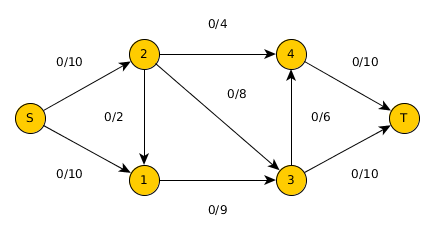
\includegraphics[scale=0.6]{dinitz/dinitz1.png}
    
\end{frame}

\begin{frame}{Ejecución}

    
    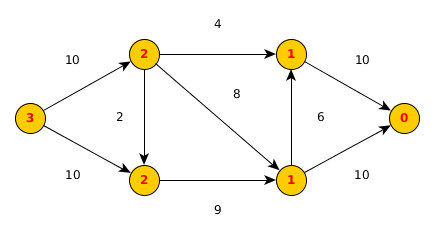
\includegraphics[scale=0.6]{dinitz/dinitz2.png}
    
\end{frame}

\begin{frame}{Ejecución}

    
    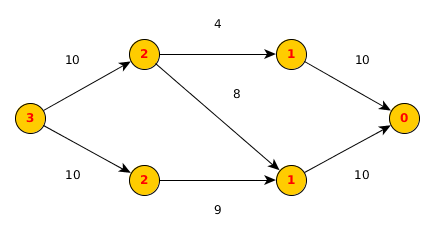
\includegraphics[scale=0.6]{dinitz/dinitz3.png}
    
\end{frame}

\begin{frame}{Ejecución}

    
    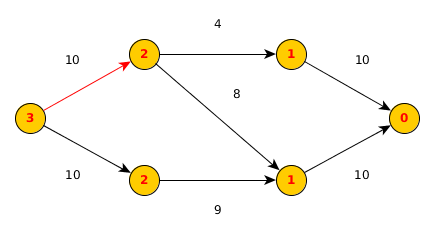
\includegraphics[scale=0.6]{dinitz/dinitz4.png}
    
\end{frame}

\begin{frame}{Ejecución}

    
    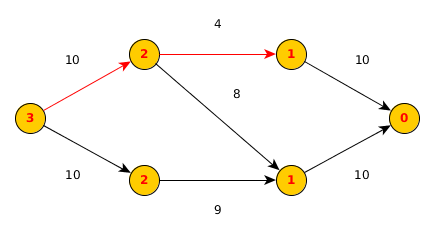
\includegraphics[scale=0.6]{dinitz/dinitz5.png}
    
\end{frame}

\begin{frame}{Ejecución}

    Recorremos el camino encontrado, pasando 4 unidades de flujo por cada arista.
    
    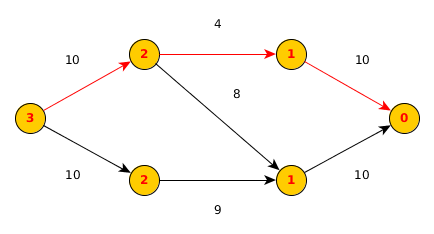
\includegraphics[scale=0.6]{dinitz/dinitz6.png}
    
\end{frame}

\begin{frame}{Ejecución}

    
    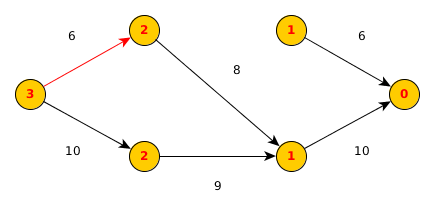
\includegraphics[scale=0.6]{dinitz/dinitz7.png}
    
\end{frame}

\begin{frame}{Ejecución}

    
    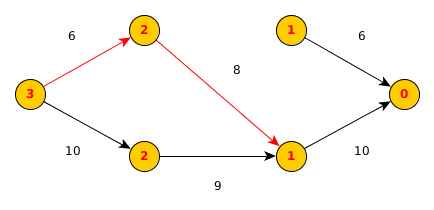
\includegraphics[scale=0.6]{dinitz/dinitz8.png}
    
\end{frame}

\begin{frame}{Ejecución}

    Recorremos el camino encontrado, pasando 6 unidades de flujo por cada arista.
    
    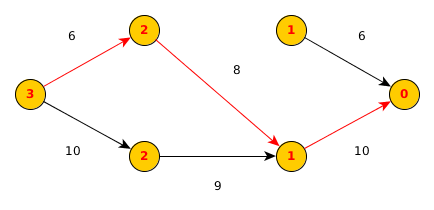
\includegraphics[scale=0.6]{dinitz/dinitz9.png}
    
\end{frame}

\begin{frame}{Ejecución}

    
    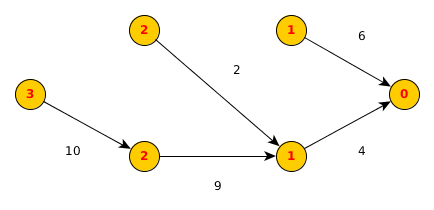
\includegraphics[scale=0.6]{dinitz/dinitz10.png}
    
\end{frame}

\begin{frame}{Ejecución}

    
    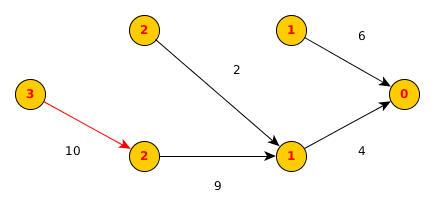
\includegraphics[scale=0.6]{dinitz/dinitz11.png}
    
\end{frame}

\begin{frame}{Ejecución}

    
    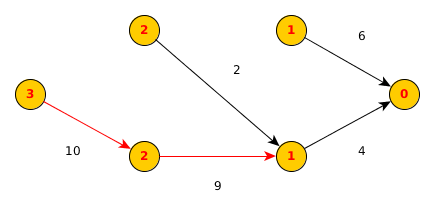
\includegraphics[scale=0.6]{dinitz/dinitz12.png}
    
\end{frame}

\begin{frame}{Ejecución}

    Recorremos el camino encontrado, pasando 4 unidades de flujo por cada arista.
    
    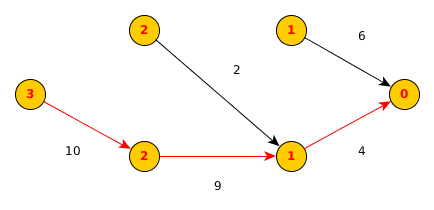
\includegraphics[scale=0.6]{dinitz/dinitz13.png}
    
\end{frame}

\begin{frame}{Ejecución}

    
    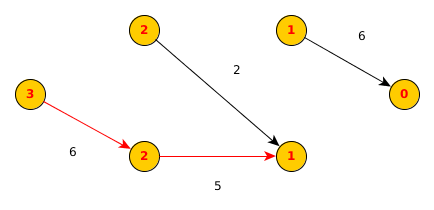
\includegraphics[scale=0.6]{dinitz/dinitz14.png}
    
\end{frame}

\begin{frame}{Ejecución}

    
    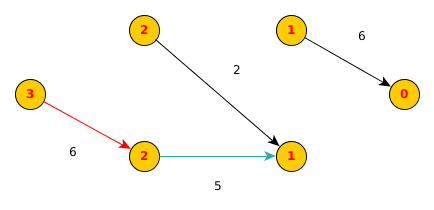
\includegraphics[scale=0.6]{dinitz/dinitz15.png}
    
\end{frame}

\begin{frame}{Ejecución}

    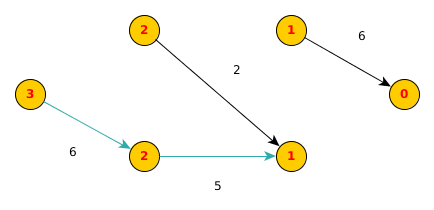
\includegraphics[scale=0.6]{dinitz/dinitz16.png}
    
\end{frame}

\begin{frame}{Ejecución}

    Flujo actual = 14
    
    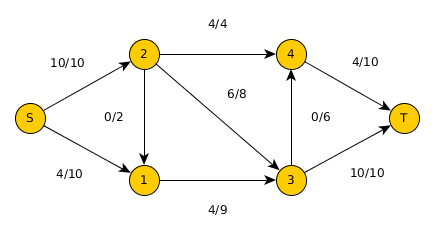
\includegraphics[scale=0.6]{dinitz/dinitz17.png}
    
\end{frame}

\begin{frame}{Ejecución}

    
    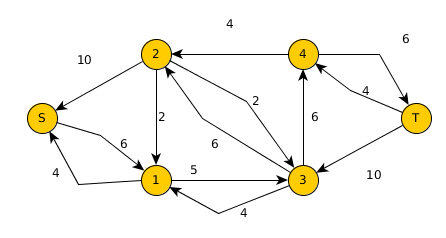
\includegraphics[scale=0.6]{dinitz/dinitz18.png}
    
\end{frame}

\begin{frame}{Ejecución}

    
    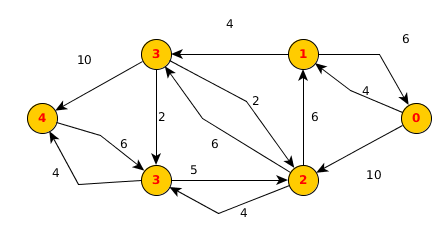
\includegraphics[scale=0.6]{dinitz/dinitz19.png}
    
\end{frame}

\begin{frame}{Ejecución}

    
    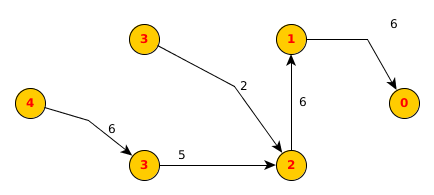
\includegraphics[scale=0.6]{dinitz/dinitz20.png}
    
\end{frame}

\begin{frame}{Ejecución}

    
    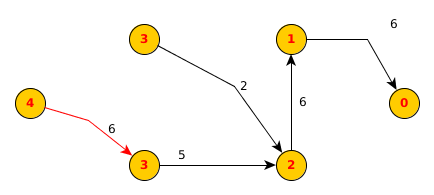
\includegraphics[scale=0.6]{dinitz/dinitz21.png}
    
\end{frame}

\begin{frame}{Ejecución}

    
    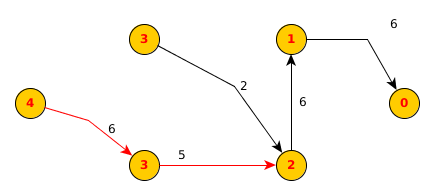
\includegraphics[scale=0.6]{dinitz/dinitz22.png}
    
\end{frame}

\begin{frame}{Ejecución}

    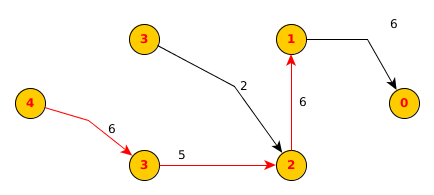
\includegraphics[scale=0.6]{dinitz/dinitz23.png}
    
\end{frame}

\begin{frame}{Ejecución}

    Recorremos el camino encontrado, pasando 5 unidades de flujo por cada arista.
    
    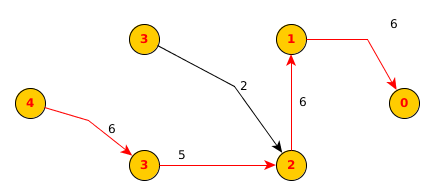
\includegraphics[scale=0.6]{dinitz/dinitz24.png}
    
\end{frame}


\begin{frame}{Ejecución}

    
    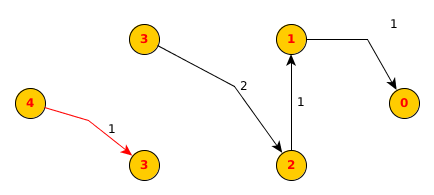
\includegraphics[scale=0.6]{dinitz/dinitz25.png}
    
\end{frame}

\begin{frame}{Ejecución}

    
    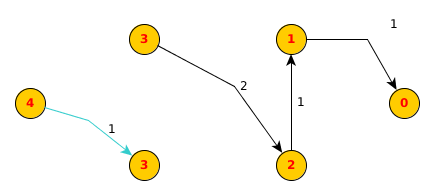
\includegraphics[scale=0.6]{dinitz/dinitz26.png}
    
\end{frame}

\begin{frame}{Ejecución}

    Flujo actual = 19.
    
    Es máximo, así que el BFS no llegará a $s$ desde $t$ ($rank(s)=\infty$).
    
    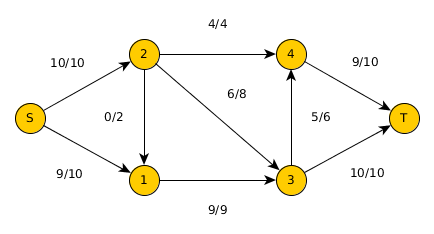
\includegraphics[scale=0.6]{dinitz/dinitz27.png}
    
\end{frame}

\begin{frame}{Complejidad}
    \begin{itemize}
        \item El algoritmo realiza $O(V)$ iteraciones, y en cada una realiza un BFS y un DFS.
        \item La complejidad \textbf{NO ES} $O(VE)$ (Esto pensó Dinitz inicialmente, antes de ir la clase de flujo máximo). ¿Por qué?
        \item En peor caso la complejidad es $O(V^2 E)$, y existen casos donde el algoritmo realiza esa cantidad de pasos.
    \end{itemize}
    \pause
    Casos especiales:
    \begin{itemize}
        \item Si todas las capacidades son 1, la complejidad es $O(min(E^{\frac{1}{2}}, V^{\frac{2}{3}}) E)$
        \item Si se usa Dinitz para resolver máximo matching bipartito, la complejidad resultante es $O(\sqrt{V} E)$
    \end{itemize}
\end{frame}

\begin{frame}{Sugerencias de implementación}
    \begin{itemize}
        \item Nunca borrar ni agregar aristas explícitamente: Con solo calcular el rank y saber el flujo (o la capacidad residual) actual, es posible saber si una arista hay que recorrerla o ignorarla.
        \item Se recorren solo las aristas con capacidad residual > 0, que van a un vecino con menor rank.
        \item Notar que DFS \textit{vuelve para atrás} al saturar un camino, con lo cual puede \textit{revisitar nodos}.
        \item Para esto es cómodo implementarlo no-recursivamente, con una pila de nodos para el camino en construcción,
                y un indicador de ``siguiente arista por considerar'' por cada nodo.
        \item Para eficiencia y practicidad, es conveniente guardar solamente la capacidad residual de las aristas.
               El flujo final puede reconstruirse de ser necesario restando las capacidades iniciales.
    \end{itemize}
\end{frame}

\begin{frame}{Referencias}
    \begin{itemize}
        \item \textit{Introduction to Algorithms, 2nd Edition}. MIT Press. \\ Thomas H. Cormen, y otros.
        \item ``\textit{Dinitz' Algorithm: The Original Version and Even's Version}'' \\ Yefim Dinitz
    \end{itemize}
\end{frame}

\end{document}
